\documentclass[tikz,border=2pt]{standalone}
\usepackage{amsmath}
\usetikzlibrary{arrows.meta}
\begin{document}
% Work in the system W(t) = [D_{A(t)} - t]^+ for A = (1,2,5,9,10), S = (3,2,1,2,2), D = (4,6,7,11,13):
% jumps by S_k at arrivals (bottom W_k, top J_k), slope -1, zero on [7,9); guide W(5) = D_3 - 5 = 2.
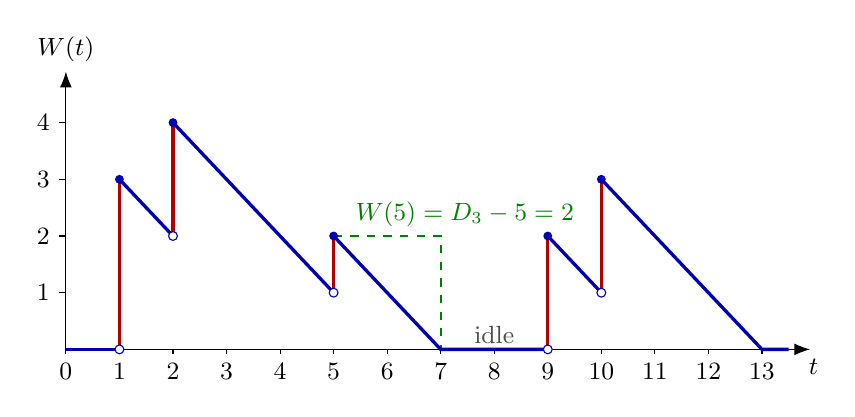
\begin{tikzpicture}[font=\small, >={Latex[length=2mm]}, x=0.68cm, y=0.72cm]
  \draw[->] (0,0) -- (13.9,0) node[anchor=north west, xshift=-4pt] {$t$};
  \draw[->] (0,0) -- (0,4.9) node[anchor=south] {$W(t)$};
  \foreach \t in {0,1,...,13} \draw (\t,0) -- (\t,-0.08) node[below] {$\t$};
  \foreach \n in {1,...,4} \draw (0,\n) -- (-0.12,\n) node[left] {$\n$};
  % guide at t = 5: the remaining work equals the time until D_3 = 7
  \draw[green!50!black, thick, dashed] (5,2) -- (7,2) -- (7,0);
  \node[green!50!black, anchor=south west, inner sep=2pt] at (5.3,2.05) {$W(5)=D_3-5=2$};
  % falling pieces with slope -1 and the idle stretches
  \draw[blue!70!black, very thick] (0,0) -- (1,0);
  \draw[blue!70!black, very thick] (1,3) -- (2,2);
  \draw[blue!70!black, very thick] (2,4) -- (5,1);
  \draw[blue!70!black, very thick] (5,2) -- (7,0) -- (9,0);
  \draw[blue!70!black, very thick] (9,2) -- (10,1);
  \draw[blue!70!black, very thick] (10,3) -- (13,0) -- (13.5,0);
  \node[gray!60!black, anchor=south, inner sep=2pt] at (8,0) {idle};
  % jumps by the service times
  \foreach \a/\lo/\hi in {1/0/3, 2/2/4, 5/1/2, 9/0/2, 10/1/3} {
    \draw[red!70!black, very thick] (\a,\lo) -- (\a,\hi);
    \draw[blue!70!black, fill=white] (\a,\lo) circle (1.6pt);
    \fill[blue!70!black] (\a,\hi) circle (1.6pt);
  }
\end{tikzpicture}
\end{document}
